\documentclass[titlepage, 12pt]{article}
\usepackage[utf8]{inputenc}
\usepackage{tabu}
\usepackage{graphicx}
\usepackage{natbib}
\usepackage{mathtools}
\usepackage{amsmath,amssymb}

% For showing hyperlinks.
\usepackage{hyperref} 
\usepackage{color}

% For showing code snippets.
\usepackage{listings}

% For formatting code.
\definecolor{codegreen}{rgb}{0,0.6,0}
\definecolor{codegray}{rgb}{0.5,0.5,0.5}
\definecolor{codepurple}{rgb}{0.58,0,0.82}
\definecolor{backcolour}{rgb}{0.95,0.95,0.92}

\lstdefinestyle{mystyle}{
    backgroundcolor=\color{backcolour},   
    commentstyle=\color{codegreen},
    keywordstyle=\color{magenta},
    numberstyle=\tiny\color{codegray},
    stringstyle=\color{codepurple},
    basicstyle=\footnotesize,
    breakatwhitespace=false,         
    breaklines=true,                 
    captionpos=b,                    
    keepspaces=true,                 
    numbers=left,                    
    numbersep=5pt,                  
    showspaces=false,                
    showstringspaces=false,
    showtabs=false,                  
    tabsize=2
}
 
\lstset{style=mystyle}


\title{Improving Incident Response of the American Red Cross in the Greater Chicago Area by Using Text Classification of Posts From Twitter}
\author{Project Members: 
\\ Manager: Pavan Sistla 
\\ Scribe/Researcher: Evan De Broux 
\\ Coder: David Cho 
\\ Coder: Christopher Millan 
\\Coder: Henry Post 
\\ Researcher/Coder: Trung Pham 
\\ Researcher: Raul Renteria 
\\ Researcher: Hasani Valdez 
\\ Researcher: Rena Haswah
}
\date{April 2019}

\begin{document}

\maketitle
\newpage
\tableofcontents
\newpage

\section{Abstract}
\hspace{0.5 cm}Tweets on Twitter about true disasters are hard to easily detect and are often hidden among a sea of irrelevant tweets about only tangentially related content. We introduce a suite of tools to obtain tweets and attempt to classify them as relevant or irrelevant with regards to house fires and other disasters using a variety of machine learning models. 

\section{Introduction}
\hspace{0.5 cm}The American Red Cross (ARC) is an organization has provided emergency assistance, disaster relief, and disaster preparedness and education across the United States since its founding in 1881. On average, the American Red Cross responds to more than 62,000 disasters a year, which is around one disaster every 8 minutes, 90 percent of which are home fires. The truly remarkable fact is that of their entire workforce that goes out of their way to help others in need, 95 percent of their workers are volunteers. In the Northern Illinois region, the ARC has received over 6,000 calls in the past 5 years and have responded to approximately 75 percent of those incidents.

\begin{figure}[h!]
\centering
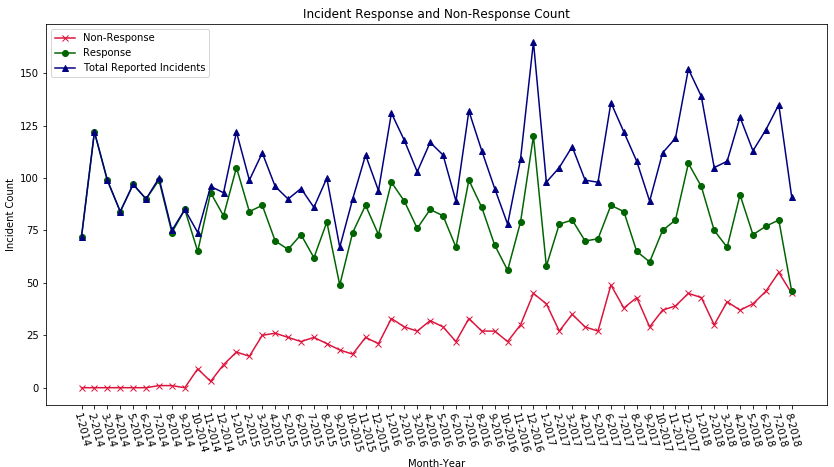
\includegraphics[scale=0.5]{pics/in_response.png}
\caption{The running count of incidents the ARC has in their records up until August 2018. We notice that despite some fluctuations in number of reported responses by month, they stay fairly steady. However, the number of incidents that the ARC did not respond to has gradually increased over this time period and additionally the ARC is unaware of many incidents in the Chicago area. Our goal is to have the ARC to be aware of more of these incidents.}
\label{fig:incident_response}
\end{figure}

\hspace{0.5 cm}Past IPRO groups who have worked for the ARC through their representative, Jim McGowan, and our instructors, Bo Rodda and Matt Robison, have given them useful insights into the data that the ARC has collected. The summer of 2018 IPRO group has shown that the fires in the City of Chicago are spatially correlated with each other. The fall of 2018 IPRO group built a fairly accurate model in predicting fires at the neighborhood level using demographic data from the Census Bureau and the City of Chicago Data Portal. This gave the ARC useful insights to answer questions such as, ``which neighborhoods should we focus our education efforts in?'' and ``which groups of people should we be targeting to better prepare them for fires?''

\hspace{0.5 cm} Despite some early exploration into the past project groups' models, there was a different point that piqued our research groups' interest. Mr. McGowan mentioned that a majority of the incidents that the ARC learns about come from social media, with specific emphasis on Twitter. During a visit on March 5th, 2019, Mr. McGowan noted that around 44 percent of the ARC's reported incidents come from Twitter. This led us to ask multiple questions. How does the ARC identify reliable sources on these social media platforms? Is it possible to evaluate the reliability of their social media sources? Can we identify new sources that report incidents, or find where fires are occurring before they are reported on more official sources? After a brainstorming session, our group came up with a potentially useful tool: a program that goes through geo-tagged tweets on Twitter and identifies those that are useful to the disaster response efforts of the ARC.

\section{Text Classification Tool}
\hspace{0.5 cm} In creating this text classification tool, there are 2 (maybe more) processes that we needed to create and fine-tune: the process of ``scraping'' the posts from Twitter and the process of classifying the tweets.
\subsection{Twitter Scraper}
\hspace{0.5 cm} The Twitter Scraper aspect of our project is a tool that simply exists to gather massive amounts of tweets with minimal effort. It exists as a Python package on the Python Package Index site, and is easily to install. Currently, it supports a handful of different methods to gather tweets.

\subsubsection{Scraping by keywords}

The first method that it can use to gather tweets is by keywords that the tweets contain. The scraper can take a single keyword and a count of results, or many keywords. Below is code showing the usage of the keyword-scraping feature:

\begin{lstlisting}[language=Python,caption=Scraping multiple keywords]
# Returns a total of 600 tweets
results = scraper.scrape_terms(
    terms={"fire", "#housefire", "firedamage"}, 
    count=200
)
\end{lstlisting}

This snippet of code will return 200 tweets each about the term ``fire'', the hashtag ``\#housefire'', and the term ``firedamage'' for a total of 600 tweets.

\subsubsection{Scraping by keywords restricted by location}

The next feature our scraper has is one which limits the areas that the scraper operates in. This is an augmentation of the scraper's ability to search for keywords and hashtags, and acts as a filter on that function.

This is important because most of the work that the ARC wishes to do takes place in or around Chicago.

Below is a code example of the same search, but restricted to within 50 miles of Chicago's center.

\begin{lstlisting}[language=Python,caption=Geo-location scraping filter]
# Returns 600 tweets that occur 50 miles from Chicago
results = scraper.scrape_terms(
    geocode="41.8297855,-87.666775,50mi",
    terms={"fire", "#housefire", "firedamage"}, 
    count=200
)
\end{lstlisting}

This time, we still get 200 tweets per term, but only ones that have been tagged within Chicago.

Instead of searching all of twitter for the three terms, only tweets that individuals have chosen to tag with a geographical location within a 50 mile radius of latitude 41.8, longitude -87.6, which is Chicago's center.

\subsubsection{Scraping by account}

This feature allows one to scrape the most recently tweeted tweets by one or more accounts.

This is to make it easy to repeatedly query accounts, or to get large amounts of tweets from a set of accounts.

Below is a code example of the scraper getting the top 100 tweets from various Twitter accounts that the  \@RedCross account follows.

\begin{lstlisting}[language=Python,caption=Scraping by account]
# Returns 300 tweets from 3 red cross accounts, 100 each.
results = scraper.scrape_accounts(
    accounts={"@RedCross", "@NWSChicago", "@MABASIllinois"},
    count=100
)
\end{lstlisting}

The syntax is very similar to that of the previous scraping methods. This snippet of code would result in a total of 300 tweets, 100 from each Twitter account.

\newpage

\subsubsection{Saving to a CSV file}

This feature allows one to save scraped tweets to a comma-separated value file, to perhaps later be analyzed in a spreadsheet program like Microsoft Excel or be loaded into another data analysis program.

\begin{lstlisting}[language=Python,caption=Saving to CSV]
# Returns 300 tweets from 3 red cross accounts, 100 each.
results = scraper.scrape_accounts(
    accounts={"@RedCross", "@NWSChicago", "@MABASIllinois"},
    count=100
)

# Saves above results to a CSV file called 'output.txt'
scraper.save_statusdict_to_csv(results, 'redcross_tweets.csv')
\end{lstlisting}

\subsubsection{Other features}

The scraper allows you to scrape many more tweets than twitter normally allows you at any one time, and will wait when it hits the Twitter API rate limit to finish scraping tweets.

\subsection{Proposed Classification Models Tested}
\subsubsection{Naive Bayes Classifer}
\hspace{0.5 cm}One of the text classification model will rely on a Naive Bayesian classifier in order to classify the tweets that we pull through Twitter's API. The tweets can be assigned a label from a finite set based on the characteristics of the tweet. The key is that the classifier will assume independence of the characteristics of the tweet, independence of the words used to construct the tweets, that would be used to determine the probability that the tweet should be assigned one of the classes.

Mathematically, the probability that a tweet would belong to a certain class, like ``fire'', is conditional. If we assume the features of the tweet are independent, have a tweet with $n$ features that are relevant to the classification of the tweet, this can be stored as a vector, $x = (x_1, x_2, ..., x_n)$. Say that there are $k$ different classes, $\{C_1, C_2, ..., C_k\}$, which the tweet could potentially be associated with. Based on the features of the tweet, we can assign a conditional probability to which class the tweet could belong to for any class $C_i, i \in \{1, 2, ... k\}$:
\begin{equation}
    P(C_i | x_1, x_2, ..., x_n)
\end{equation}

The obvious problem with this line of thinking is that the number of features for a tweet can be relatively large, well as many features as you can fit into 280 characters anyway. Using Bayes' Theorem, the probability a tweet being associated with class $C_i$, would be:

\begin{equation}
    P(C_i | x) = \frac{p(C_i)p(x|C_i)}{p(x)}
\end{equation}
In other words, the probability that a tweet belongs to class $i$ is equal to the prior likelihood that a tweet belonged to class $i$ times the likelihood probability that this tweet belongs to class $i$, divided by the likelihood that the specific tweet exists in that order. Note that the numerator is really the only thing of interest here, as it is dependent on class $k$. Using the laws of conditional probability, we can rewrite the joint probability of the model:

\begin{equation}
    P(C_i, x_1, ..., x_n) = P(x_1|x_2, ...,x_n, C_k) P(x_2,...,x_n, C_k)
\end{equation}
\begin{equation}
    =P(x_1|x_2, ..., x_n, C_k)P(x_2|x_3, ..., x_n, C_k)P(x_3, ..., x_n, C_k)=...
\end{equation}
\begin{equation}
    =P(x_1|x_2,..., x_n, C_k)P(x_2|x_3,..., x_n, C_k) ...P(x_n|C_k)P(C_k)
\end{equation}
Yet, naive conditional independence implies that for any feature $x_j$ is conditionally independent of $x_l$, for any $j \neq l$, which translates to:
\begin{equation}
    P(x_j| x_{j+1}, ..., x_n, C_k) = P(x_j|C_k)
\end{equation}
This changes the conditional probability to:
\begin{equation}
    P(C_k|x_1, ..., x_n) \propto P(C_k, x_1, ..., x_n)
\end{equation}
\begin{equation}
    =P(C_k) \prod_{i=1}^{n} P(x_i|C_k)
\end{equation}
Using the independence assumptions, the probability of observing class $C_k$, given features $\{x_1, ..., x_n\}$ is:
\begin{equation}
    \frac{P(C_k) \prod_{i=1}^{n} P(x_i|C_k)}{P(x_1, ..., x_n)}
\end{equation}
\begin{equation}
    =\frac{P(C_k) \prod_{i=1}^{n} P(x_i|C_k)}{\sum_{k}P(C_k)P(x_1, x_2,..., x_n|C_k)}
\end{equation}
\hspace{0.5 cm}This is how probabilities are solved for using any distribution to determine $P(C_k|x_1, ..., x_n)$. We are using the multinomial distribution to determine the class probabilities. This means that $P(x_1, ..., x_n|C_k)$ is written as:
\begin{equation}
    P(x_1, ..., x_n|C_k) = \frac{(\sum_i x_i)!}{\prod_i x_i!}\prod_i p_{ki}^{x_i}
\end{equation}
where $p_{ki}$ is the probability of class $k$ associated with observation $i$.

\subsubsection{Logistic Model}
\hspace{0.5 cm}Logistic regression model classification are fairly simple. Define a single logistic response variable to be $y_i$, which is an ordinary Bernoulli random variable, i.e. a binary response variable that can take on values of 0 or 1, with:

\begin{equation}
    P(y_i = 1) = \pi_i
    P(y_i = 0) = 1 - \pi_i
\end{equation}

which means $y_i$ has a probability distribution of:
\begin{equation}
    f_i(y_i) = \pi_i^{y_i}(1-\pi_i)^{1-y_i}, \forall i =1,...,n
\end{equation}

which after compiling all $y_i$ for $i = 1, 2, ..., n$ assuming independence between observations $y_i$ has joint probability distribution:
\begin{equation}
    g(y_1, ..., y_n) = \prod_{i=1}^{n} f_i(y_i)= \prod_{i=1}^{n}\pi_i^{y_i}(1-\pi_i)^{1-y_i}
\end{equation}.
To find the maximum likelihood estimates of the probability we can utilize the logarithmic transformation:
\begin{equation}
    ln(g(y_1, ..., y_n)) =\sum_{i=1}^{n} y_i ln(\frac{\pi_i}{1-\pi_i}) + \sum_{i=1}^{n}ln(1-\pi_i)
\end{equation}
which yields:
\begin{equation}
    1-\pi_i = \frac{1}{1+e^{\beta_0 + \beta_1x_{i1} + ... + \beta_{n-1}x_{i,n-1}}} 
\end{equation}
\begin{equation}
    \rightarrow ln(\frac{\pi_i}{1-\pi_i})=\beta_0 + \beta_1x_{i1} + ...+\beta_{i,n-1}x_{i, n-1}
\end{equation}
This quantity on the right outputs a probability that $y_i$ occurs given the observed independent variables $x_{i1}, ..., x_{i, n-1}, \forall i \in \{1,..., n\}$.
\citep{alsm.2005}

\hspace{0.5 cm}However, the case above does not involve multiple responses, or polytomous logistic regression for nominal responses, but a single response. This is necessary as we have multiple categories, but it also complicates the mathematics. Say we have $J$ different responses categories, where $y_{ij} \in \{0,1\}$, which is the case where case $i$ has response $j$. We assume that only one category can be selected for response:

\begin{equation}
    \sum_{j=1}^{J} y_{ij} =1
\end{equation}
We let the probability that case $i$ is in category $j$ be represented by $P(y_{ij} = 1) = \pi_{ij}$. For $J$ polytomous categories, there would be $J(J-1)/2$ pairs of categories and thus the same amount of linear predictors of form:

\begin{equation}
    \pi'_{ij'j} = ln(\frac{\pi_{ij'}}{\pi_{ij}}) = X_i'\beta_{j'j}, \forall j'<j; j',j \in \{1,..., J\} 
\end{equation}
If we assume a baseline, like the ``NO'' category that classifies tweets that are irrelevant to our search, then we can treat this as class $J$ and we know that the logits for the $J^{th}$ comparison are:
\begin{equation}
    \pi'_{ijJ} = ln(\frac{\pi_{ij}}{\pi_{iJ}}) = X_i'\beta_{jJ}, \forall j \in \{1,2,...,J-1\}
\end{equation}
Since the comparisons are being made against this baseline, we assume these probabilities are now:
\begin{equation}
    \pi_{ij}' = ln(\frac{\pi_{ij}}{\pi_{iJ}}) = X_i'\beta_j, \forall j \in \{1, ..., J-1\}
\end{equation}
We can always find the difference in any two responses from these $J-1$ logits as for any $k \neq l$:
\begin{equation}
    ln(\frac{\pi_{ik}}{\pi{il}}) = ln(\frac{\pi_{ik}}{\pi_{iJ}} * \frac{\pi_{iJ}}{\pi_{il}}) = X_i'\beta_k - X'_i\beta_l
\end{equation}
This yields the $J-1$ logit expressions for the category probabilities in case $i$:
\begin{equation}
    \pi_{ij} = \frac{e^{X_i'\beta_j}}{1 + \sum_{k=1}^{J-1} e^{X_i'\beta_k}}, \forall j \in \{1, ..., J-1\}
\end{equation}
\citep{alsm.2005}

\subsubsection{Linear Support Vector Classification}
\hspace{0.5 cm}We will define how a linear support vector machine works mathematically in a simple case. Say we have a set of training data $(x_i, y_i), \forall i \in\{1,...,n\}$. The only values that $y_i$ can take on are 1 or -1 which classifies the data $x_i$ (the support vectors) into one of two classes, where $x_i$ has dimension $p$. There will be some "maximum margin hyperplane" such that we can divide the data into the two classes for which the distance from the hyperplane to the nearest vector $x_i$ is maximized. It is possible to write any hyperplane for a set of points $x$ as:

=\begin{equation}
    w\cdot x - b = 0
\end{equation}
where $w$ and $x$ are vectors of the same dimension and $b$ is a real number. $w$ is the normal vector to the hyperplane. It is probably safe to assume that the data that we have been given is linearly separable. Given this, the data could be standardized to satisfy the equations one of the two equations:
\begin{equation}
    w \cdot x - b = 1, 
\end{equation}
or:
\begin{equation}
    w \cdot x - b = -1
\end{equation}
depending on the classification of the data. The data also cannot fall into this ''hard margin'', so we need to add two constraints on the data:
\begin{equation}
    w \cdot x - b \geq 1, given: y_i = 1
\end{equation}
\begin{equation}
     w \cdot x - b \leq -1, given: y_i = -1
\end{equation}
This can be turned into a linear optimization problem:

\begin{alignat*}{2}
 \text{minimize: }  ||w||  &\\
  &\text{subject to: } \displaystyle y_i(w \cdot x - b) \geq 1, i=1 ,..., n &\\
        &y_{i} \in \{0,1\}, j=1 ,..., n
\end{alignat*}{2}

\hspace{0.5 cm}If the data is not linearly separable, then a ''soft margin'', then we have a loss function which tries to compensate for this lack of separation:
\begin{equation}
    max\{0, 1 - y_i(w_i \cdot x_i - b)\}
\end{equation}
and we wish to minimize the function:
\begin{equation}
    [\frac{1}{n}\sum_{i=1}^{n} max\{0, 1 - y_i(w_i \cdot x_i - b)\}]+\lambda||w||^2,
\end{equation}
where $\lambda$ is a parameter that weights the trade-off of increasing the margin side so that the independent data vector $x_i$ is on the correct side of the margin. Although the problem described here uses only two classes to try to define these margins, we can generalize these arguments to an n-dimensional hyperplane.

\section{Data Sources}

\subsection{Classified Tweets}
\hspace{0.5 cm}In order to train this model we needed collect reliably classified tweets. In order to do this, we gained access to a dataset of approximately 2.5 million classified tweets from Axel Schulz and Christian Guckelsberger which had classified  tweets into multiple categories, ``fire'', ``shooting'', ``crash'', and ``no'' for neutral. We used a subset of these tweets that were associated with locations in Chicago, New York, Boston, Memphis, and Seattle, as the types of incidents could be assumed to be similar across these 4 metropolitan areas and the local vernacular for describing these incidents should vary a great deal across these American cities. Due to an imbalance in the number of incidents in the ''crash'' and ''flood'' categories, we decided to focus on classifying the ''NO'', ''fire'', and ''flood'' categories.
\citep{CT.2015}

\subsection{Twitter API}
\hspace{0.5 cm}In order to even classify tweets in the first place, we needed to pull tweets from Twitter. Since we are associated with an educational institution, we were able to pull 1500 tweets at a time every 15 minutes. Specifically, we tried to find tweets that were geo-tagged to help the ARC identify the location of incidents. These tweets would be stored on a MongoDB database, and could be pulled by query.

\subsection{UCI Machine Learning Respository: Humanitarian Data}
\hspace{0.5 cm}This is a sample of social media posts from Twitter and Instargram collected by researchers from the University of Beirut. We used some 600 tweets that classified fires and floods from these social media platform which should improve the reliability of the text classification model's performance.
\citep{UCI.2016}

\section{Results: Text Classification Performance}
\begin{figure}[h!]
\centering
\includegraphics[scale=0.8]{pics/tw_po_by_cat.jpg}
\caption{Number of tweets in each category used in training the model.}
\label{fig:classified_tweet_count}
\end{figure}

\subsection{Scraper Alone}
\hspace{0.5 cm}In early April 2019, Henry Post used our Twitter scraping tool to pull over 1,100 tweets geo-tagged 20 miles around Chicago without re-tweets in the dataset that keyword searched ''fire'', ''house fire'', ''mudslide'', ''landslide'', and ''emergency''. We eliminated ''landslide'' and ''mudslide'' from the dataset as Chicago is at an extremely low risk of having these events occur so close to Chicago. After eliminating this data, we manually parsed through every tweet to determine if it was a viable incident that the ARC could respond to. After over an hour of work, only a handful of tweets were classified as one of the categories used in the models. Although this did not take a significant amount of time or human-power to finish the task, if you remove the geo-tagged restriction on the scraped tweets this task becomes unfeasible.
\subsection{Comparing Model Performance}

\begin{figure}[h!]
\centering
\includegraphics[scale=0.5]{pics/results_large_text.png}
\caption{Results depicting the accuracy of the 4 classification models tested.}
\label{fig:model_results}
\end{figure}\\

\hspace{0.5 cm}We then evaluated the data we received from Schulz and Guckelsberger \citep{CT.2015} along with the UC-Irvine dataset \citep{UCI.2016} to train a model using each of the three methods described earlier in the paper using an 80/20 split of training data and test data from these datasets. We additionally used a random forest classifier to try to classify the tweets.\\

\begin{figure}[h!]
\centering
\includegraphics[scale=0.5]{pics/confusion.png}
\caption{The confusion matrix for the dataset being run through the model. The squares in the upper right represent the number of false negatives for each classification, the bottom left squares represent the false positives for each of the classifications, and the squares on the diagonal represent the number of true positives/negatives for each classification.}
\label{fig:confusion_matrix}
\end{figure}\\

There were four different types of models that were under consideration. Clearly, the random forest classifier was the least accurate classifier of the four models tested. The LinearSVC model showed the highest accuracy, and thus we will choose to use the LinearSVC model to classify the tweets into the incident categories. (\ref{fig:model_results})\\

 The confusion matrix (\ref{fig:confusion_matrix}) shows not only the accuracy of the model, but also where the models misclassified the most, and what categories the models misclassified to. These results are based off tweets the model has never seen before. The model reads the text and outputs a prediction for that text, the bottom side labeled Predicted; either ''fire'', ''flood'', or ''NO''. Then it compares it to its actual label, the left side that says Actual. The matrix shows that out of all the tweets in the test data set, the model correctly classified 108 as ''fire'', 115 as ''flood'', and 412 as ''NO'', our neutral class.\\
 
 \begin{figure}[h!]
\begin{center}
\begin{tabu} to 0.9\textwidth { | X[c] | X[c] |X[c] |X[c] |}
 \hline
  Actual $\downarrow$/ Predicted $\rightarrow$& Fire & Flood & NO/Neutral \\
 \hline
  Fire & 108 & 2 & 38  \\
 \hline 
 Flood & 1 & 115 & 11 \\
 \hline
 NO/Neutral & 0 & 0 & 412 \\
 \hline
\end{tabu}
\end{center}
\caption{We see that the the LinearSVC model does well correctly classifying fire and flood social media posts. However, there is some difficulty in the classification of the neutral class.}
\end{figure}
 
\begin{figure}[h!]
\centering
\includegraphics[scale=0.5]{pics/stats.png}
\caption{Quantitative measurements of the model evaluating accuracy of categorical classifications.}
\label{fig:stats}
\end{figure}\\

We chose to analyze the precision and recall scores of the models as these essentially measure the true positive rate of the model (\ref{fig:stats}). Precision is equal to the true positive results over the divided by the number of true positive and false positive results, in other words the total number of correctly classified tweets over total number of predicted positive tweets. Precision gives an indication of the what percentage of tweets are returned by the model that are actually relevant to the search. Recall is the true positive over the total number of true positive and false negative results, or the number of correctly classified tweets over the total number of tweets that were actual positives. On the other hand, recall refers to the percentage of total relevant results correctly classified by our algorithm. 

\hspace{0.5 cm}The F1-score is defined to be:
\begin{equation}
    F_1 = 2 * \frac{precision * recall}{precision+recall}
\end{equation}
simply the harmonic mean of precision and recall. It could be seen as a weighted accuracy score, as it weights the accuracy if the categories are not balanced, which in this case they are. Overall the model performs decently given the current scores and the f1-score. A way to maximize the recall would be to perform the active learning part of the project, meaning it will begin to correctly classify tweets that are more similar to the ones the ARC would see, than just generic ones from our dataset. 

\section{Conclusion}
\hspace{0.5 cm}Over the course of the semester, this IPRO group was able to build a tool that could keyword search or account search Twitter to find potentially relevant tweets that the ARC could use for their incident response. Despite having the power of this tool, it was found to have too many irrelevant tweets to manually parse through to be useful on its own. The research groups' work of finding machine learning classification algorithms to implement into the scraper proved successful in accurately and precisely analyzing social media posts from Twitter and placing them in the correct category. The analysis of the models that were tested led the group to select the `LinearSVC` classifier to analyze the tweets.
% This is probably too short

\section{Future Work}
% Add a section on integration with the machine learning tool?

\subsection{False Positives and Active Learning Strategy}

\hspace{0.5 cm}The general problem of active learning can be described in this case as follows: there is a set of tweets that our scraper will identify at some time $i$, where $i \in \{1, 2,..., n\}$ and is a period of time, hour, day, week, etc. We have a set of total tweets, $T$. At each time period, we will have 3 types of tweets:
\begin{enumerate}
    \item A set of tweets that already has a known classification, say this subset is called $T_{L,i}$, where the subscripts stand for labeled at time $i$.
    \item A set of tweets that has an unknown classification, call this subset $T_{U,i}$.
    \item A set of the tweets that has been picked to be labeled by the ARC or our program, say this subset is $T_{P,i}$.
\end{enumerate}
The goal is to pick the best tweets for the third set $T_{P,i}$. In this case, the text classification model will have provided a first type of label, the type of incident the text classifier has associated with the tweet. Now, the ARC may be able to provide two types of labels to these tweets.
\begin{enumerate}
    \item If the tweet's classification label was correct.
    \item Whether or not the tweet was used in a response to an incident.
\end{enumerate}
\hspace{0.5 cm}In response to the first item, our historical database of tweets is fairly large, so it seems unlikely that the classifications would be incorrect. However, given the prevalence of bots and other trolls that could produce seemingly authentic text, the ARC may want to identify these false positives. Second item is also of interest, as it would be ideal if the ARC would also provide the model with tweets that it found to be useful. 

\hspace{0.5 cm}Although the issue with false positives is important, we can reframe the issue to make the two problems one. The model will be identifying tweets that are thought to be positive. We will make two assumptions. One is that the false positives and true positives pulled by our Twitter scraper/classification tool do not have the wrong incident type label. An incident could be a false positive, this is true, but we are assuming that if something has an initial label, say ``fire'', then it will not be reclassified as a different incident type, such as ``flood''. The second is that the  that it is likely that the ARC would be able to find multiple reports of incidents when deciding on whether or not they should respond to the incident, from OEMC, IPN, or radioman911. The ARC contacts the local jurisdiction to see if they can be of assistance to an incident as well. This active classification would require an ARC volunteer to label the outputs from the scraper, and then to label the tweet as ``True'' or ``False'', i.e. the tweet was useful or the tweet was a false flag. This would be a scenario of stream-based selective sampling, as the tweets the model draws from Twitter are drawn one at a time from Twitter by the model \citep{settles.tr09}. The ability to confirm or refute an incident report is vital to being able to actively train the model.

\hspace{0.5 cm}From the tweets the scraper does receive, there will be a selection of which tweets the ARC uses. We propose the addition of these tweets to the database. The issue becomes if the ARC does not use tweets, but they are still true positives when identifying incidents, we do not want to simply label these as false positives. These classifications will ``confuse'' the model.

\hspace{0.5 cm}The decision whether or not to query new tweets that are pulled by the classifier can be handled in a few ways. One could try to query using an ``informativeness measure, and make a biased random decision, such that more informative instances are more likely to be queried'' \citep{settles.tr09}.

\subsection{Evaluating Reliability}

\hspace{0.5 cm}Once the tweets are stored to our database, it may not only be useful to train our program to identify incidents from Twitter using new tweets/social media posts that it has labeled as corresponding to an incident in the Northern Illinois region, but it may be smart to keep track of accounts that are viewed as more useful in aiding the ARC's responses. This would perhaps require a ranking of accounts where accounts have been selected by the scraper, and a way to score the usage of these accounts' tweets for when they are selected for use by the ARC. For this, we propose two simple measures for these two account traits:
\begin{enumerate}
    \item Actively keeping track of the number of times a certain account is identified by the Twitter scraper
    \item We then will keep track of a percentage of the number of times an account had their tweets used by the ARC when selected by our model out of the total number of times the scraper selects a tweet from Twitter. If we were to make this a graphic, it may not be smart only to rank by percentage, as accounts that have popped up once and were selected in that one appearance may dominate the rankings. Hence, we will set a threshold tweets. If an account has been selected by the scraper a certain amount of times, it will become eligible to enter the percent usage rankings.
\end{enumerate}

This is the most complex measure, but future groups could look at finding or developing measures of accuracy and/or precision to implement into the dashboard and analysis.
\bibliographystyle{plain}
\bibliography{references}
\end{document}